%%% Compile with LuaLaTeX and TeXLive for best results
\documentclass[	ignorenonframetext,%
		 		boxes,%
				xcolor=dvipsnames,%
				14pt]{beamer}
\usepackage{multimedia}
\def\beamerforarticle{y} % set to y if creating a presentation for inclusion in handouts, n otherwise
% the snm file has to be edited for the article to be generated correctly in a separate process
%\def\beamerforarticle{n} % set to nH if creating a stand alone presentation with real animations
%% Author: 		Pablo Adames
%% Date:			June 16, 2013 (first created as template-contents.tex)
%%				Nov 6, 2013 (second version for Schlumberger )
%%				Nov 15, 2013 (handout version for Schlumberger)
%%				Apr 03, 2014 (first version TUFFP presentation, added documentation on usage)
%%              Aug 09, 2019 (CalgaryR meetup)
%%              Mar 02, 2022 (CDMA2022 paper)
%%
%% File:			ComparisonFrigssStFergusFlowModelsTUFFPApr082014.tex
%%
%% Notes:		This file is compilable using LuaLaTeX and TeXlive for best results
%%
%%				This file is to be the placeholder of
%%				the structure of either a presentation with
%%				fully functional slides or an article with the slides
%%				plus comments for completeness.
%%
%%				The presentation may have animations, movies, and other features
%%				that are meant to be shown in full screen mode.
%%
%%				The article is supposed to be the documentation accompanying the
%%				full featured presentation. It will have all the sildes in smaller
%%				size for reference plus all the contextual information to
%%				allow interpretation of the presentation slides in a logical
%%				sequence from beginning to end.

%% Usage:		First compile the following file using LuaLaTeX and TexLive:

%%				`PresentationComparisonFrigssStFergusFlowModelsVMGNov2014.beamer.tex'
%%
%%					\documentclass[	ignorenonframetext, boxes, xcolor=dvipsnames, 14pt]{beamer}
%%					\usepackage{multimedia}
%%					\def\beamerforarticle{n}
%%					\input{PresentationComparisonFrigssStFergusFlowModelsVMGNov2014}

%%				This will generate the PDF from the beamer presentation LaTeX markup
%%				Then compile the following file using LuaLaTeX and TexLive:

%%				`PresentationComparisonFrigssStFergusFlowModelsVMGNov2014.article.tex'

%%					\documentclass[12pt,letterpaper]{article}
%%					\usepackage[activeospeccharacters]{beamerarticle}
%%					\usepackage[top=2cm,bottom=2cm,left=2.5cm,right=2cm]{geometry}
%%					\usepackage[labelfont=bf,textfont={sl,bf},lofdepth,lotdepth]{subfig}
%%					\setjobnamebeamerversion{PresentationComparisonFrigssStFergusFlowModelsVMGNov2014.beamer}
%%					\input{PresentationComparisonFrigssStFergusFlowModelsVMGNov2014}
%%
%%				That will produce the PDF as an article with the slides
%%				in it as scaled down graphics.
%%				Note: you may have to edit the file:
%%				`PresentationComparisonFrigssStFergusFlowModelsTUFFPApr082014.beamer.snm'
%%				to number the repeated slide numbers of consecutive overlayed slides to
%%				be able to repfer to them appropriately in the article version.
%\usetheme{default} % will use "boxes" as specified in the '\documentclass[]{}' command
%\usetheme{Boadilla}% ok
\usetheme{CambridgeUS}% best (mod template by raising logos to allow for footnote template)
%\usetheme{EastLansing} % green version of 'CambridgeUS'
%\usetheme{Goettingen}% pretty good if right side bar is ok...would have to remove the top navigation from slide Configuration
%\usetheme{Malmoe}% dark colours, after changing configuration slides looks better
%\usetheme{Marburg}% side bar, strong colours, similar to 'Goettingen'
%\usetheme{Montpellier}%LOVE IT, very descrete top navigation guide
%\usetheme{Szeged}% LOVE IT TOO, similar to Montpellier but footnote and top navigation has different structure
%\usetheme{Warsaw}% Singapore, Szeged, Warsaw
%\usepackage[autoplay,draft]{animate}%set final locally at each animation
\usepackage[export]{adjustbox}
\usepackage[autoplay,final]{animate}%set draft locally at each animation
\usepackage{caption}
\captionsetup[figure]{font={small,it,bf},labelfont={small,it,bf}}
\usepackage{tikz} % to make circled numbers in personal commands file and data flow diagram
\usetikzlibrary{arrows}
\usetikzlibrary{shapes.geometric}
\usetikzlibrary{positioning}
\usetikzlibrary{decorations.text,decorations.shapes, arrows.meta, decorations.pathreplacing,decorations.pathmorphing}
\usetikzlibrary{bending,arrows.meta,patterns,calc,fit}
\usepackage{tkz-euclide}

\usepackage{pgfplots}

\pgfplotsset{compat=1.9}
\pgfplotsset{donleft/.style={%
        scale only axis,
        xmajorgrids,
        xlabel = {Minimum number of donations per user},
        axis y line*=left,
        ylabel style = {align=center},
        ylabel     = {Transactions, $\times$ 10\textsuperscript{6} \ref{pgfplots:nt}},
        xtick      = {1,50,100,200, 300,400,500},
        ytick      = {0,2,5,10,15,20,25},
        width = 6.2cm }}
\pgfplotsset{donlogright/.style={%
        log y ticks with fixed point,
        scale only axis,
        axis x line=none,
        axis y line*=right,
        ylabel style = {align=center},
        ylabel       = {Users, $\times$ 10\textsuperscript{3} \ref{pgfplots:users}},
        xtick      = {1,50,100,200, 300,400,500},
        ytick      = {1,10,100,1000},
        width = 6.2cm }}
\pgfplotsset{comleft/.style={%
        scale only axis,
        axis x line=none,
        axis y line*=left,
        ylabel style = {align=center},
        ylabel       = {Causes, $\times$ 10\textsuperscript{3} \ref{pgfplots:cause}},
        ytick      = {0,25,50,75,100,125,150,175},
        xtick      = {1,50,100,200, 300,400,500},
        width = 6.2cm }}
\pgfplotsset{comright/.style={%
        scale only axis,
        xmajorgrids,
        xlabel = {Minimum number of donations per user},
        axis y line*=right,
        ylabel style = {align=center},
        ylabel     = {Companies, \ref{pgfplots:cmp}},
        xtick      = {1,50,100,200, 300,400,500},
        ytick      = {0,50,100,150,200,250,300,350,400},
        width = 6.2cm }}
\pgfplotsset{cntyleft/.style={%
        scale only axis,
        grid       = both,
        xlabel     = {Minimum number of donations per user},
        ylabel style = {align=center},
        ylabel     = {User countries, \ref{pgfplots:usrcnty}},
        xtick      = {1,50,100,200, 300,400,500},
        width = 6.2cm }}
\pgfplotsset{mapfigs/.style=,
        xlabel = {Top-k recommendations},
        ymin = 5,
        ymax = 35,
        xtick = {3,4,...,11},
        ytick = {5,10,15,20,25,30,35}}}


\usepackage{pstricks,pst-plot}
% \usetikzlibrary{shapes,arrows,decorations.markings,decorations.pathmorphing,decorations.text}
% \usetikzlibrary{bending,arrows.meta,patterns,calc,fit}
% \usetikzlibrary{decorations.pathreplacing}
%\usetikzlibrary{positioning-plus,node-families}
% \usepackage{tkz-euclide}
%\usetikzlibrary{mindmap}
\renewcommand{\familydefault}{\sfdefault}
\usepackage{helvet}
\usepackage{fontspec} % Please compile using LuaLaTeX if using these two lines...
%\setmainfont{Arial} % otherwise switch to the previous helvet package and use pdfLaTeX
%\usepackage{multimedia}
\mode<article>{ \usepackage{paralist} }
\usepackage{pgfkeys }
\usepackage{fancybox}
\usepackage{amsmath}
\usepackage{amssymb}
\usepackage{amsfonts}
\usepackage{tabularx}
\usepackage{booktabs}	  	%design of table, has an excellent documentation
\usepackage{multirow}
\usepackage{calc} % to combine measures in textpos commands for instance
\usepackage[absolute,overlay]{textpos}
% \usepackage[texcoord,grid,gridcolor=red!10,subgridcolor=green!10,gridunit=pt]{eso-pic}
\usepackage{fontawesome}
\usepackage{savesym}
\savesymbol{checkmark}
\usepackage{dingbat}
\restoresymbol{DINGBAT}{checkmark} % avoids collision with definition in ams package

\usepackage{textcomp}
\usepackage{array}
\usepackage{threeparttable}
\usepackage{microtype} % for awesome spacing and a pleasant look
\usepackage{dblfloatfix}
\usepackage[ruled,vlined]{algorithm2e}

%\usepackage[absolute,overlay,showboxes]{textpos}
\usepackage{hyperref}
%\definecolor{slbheadings}{RGB}{0,51,102}%blue
\definecolor{slbheadings}{RGB}{0.07,0.32,0.30}%deep jungle green (https://rgbcolorcode.com/color/4DA6FF)

\hypersetup{%
    colorlinks=false,
    linkbordercolor = {blue!20!black!60!red},
    breaklinks,
    linkcolor=blue!20!black!60!red,
    urlcolor=slbheadings,
    anchorcolor=blue!20!black!60!red,
    citecolor=blue!20!black!60!red}
\hypersetup{%
    pdftitle={Recommendation System to Suggest Charities without Explicit User Profiles Using Dual-AutoEncoders},
    pdfauthor={Pablo E. Adames},
    pdfsubject={A presentation for Data4Good Meetup Apr 28 2022},
    pdfcreator={\LaTeX\ with package \flqq hyperref\frqq and document class \flqq beamer \frqq},
    pdfkeywords={recommendations, auto-encoders, donations, relevance},
    pdfproducer={LuaLaTeX}%
}


\definecolor{headings}{RGB}{0,0,0}%Black
\definecolor{fgbox}{rgb}{0.2,0,0.2} % dark midnight blue
\definecolor{bgbox}{rgb}{0,0.4,0.6}
%\definecolor{text}{rgb}{0,0.2, 0.4}
\definecolor{text}{rgb}{0.07,0.32,0.30} % deep jungle green


\definecolor{amazon}{rgb}{0.23,0.48,0.34} %3A7A57 Sea green
\definecolor{amazonlight}{rgb}{0.62,0.74,0.67}
\definecolor{amazonComp}{rgb}{0.48,0.23,0.37}



\mode<article>{
    \usepackage[automark,headsepline,footsepline]{scrlayer-scrpage}
    \setheadsepline{2pt}[\color{orange}]
    \setfootsepline{2pt}[\color{orange}]
}

\mode<beamer>{
    \setbeamercovered{transparent}
    

\setbeamertemplate{navigation symbols}{}
% \addtobeamertemplate{headline}{%
%     \leavevmode%
%     \hbox{\begin{beamercolorbox}[%
%             wd=0.9\paperwidth,
%             ht=2.5ex,
%             dp=1.125ex,
%             right,
%             leftskip=.3cm,
%             rightskip=.3cm plus1fil] {title in head/foot}%
%             \usebeamerfont{title in head/foot}\insertsectionnavigationhorizontal{0.9\paperwidth}{}{\hskip0pt plus1filll}
%         \end{beamercolorbox}
% %        \begin{beamercolorbox}[%
% %            wd=0.1\paperwidth,
% %            ht=2.5ex,
% %            dp=1.125ex,
% %            right,
% %            leftskip=.3cm,
% %            rightskip=.3cm plus1fil] {title in head/foot}%
% %            \usebeamerfont{title in head/foot} \insertframenumber/\inserttotalframenumber
% %        \end{beamercolorbox}}%
% }
%     \vskip0pt%
%     \hbox{\begin{beamercolorbox}[%
%             wd=0.9\paperwidth,
%             ht=2.5ex,
%             dp=1.125ex,
%             right,
%             leftskip=.3cm,
%             rightskip=.3cm plus1fil] {title in head/foot}%
%             \usebeamerfont{title in head/foot}\insertsubsectionhead
%         \end{beamercolorbox}%
% }}

%% commented out afteer switching from beamer theme 'Montpellier' to 'CambridgeUS'
%% the numbering comes with the theme in a bottom footer
% \addtobeamertemplate{footline}{%
%     \leavevmode%
%     \vspace{5.7ex}\hspace{0.45\paperwidth}%places them near the center of the page
%     \hbox{\begin{beamercolorbox}[%
%             wd=0.1\paperwidth,
%             ht=2.5ex,
%             dp=1.125ex,
%             right,
%             leftskip=.3cm,
%             rightskip=.3cm plus1fil] {footline}%
%             \usebeamerfont{footline} \insertframenumber/\inserttotalframenumber 
%         \end{beamercolorbox}}%
%     \vskip0pt%
% }        



        % From: http://tex.stackexchange.com/questions/137022/how-to-insert-page-number-in-beamer-navigation-bars
        
%\addtobeamertemplate{navigation symbols}{} 
%        \addtobeamertemplate{footline}{%
%            \leavevmode%
%                        \vspace{5.7ex}\hspace{1.6em}%
%            \hbox{\begin{beamercolorbox}[%
%                    wd=0.5\paperwidth,
%                    ht=2.5ex,
%                    dp=1.125ex,
%                    right,
%                    leftskip=.3cm,
%                    rightskip=.3cm plus1fil] {footline}%
%                    \usebeamerfont{footline} \insertframenumber/\inserttotalframenumber 
%                \end{beamercolorbox}}%
%                \vskip0pt%
%            }

    % \setbeamertemplate{title page}[default]
    \setbeamercolor{normal text}{fg=text,bg=white}
    \setbeamercolor{alerted text}{fg=amazonComp}
    \setbeamercolor{example text}{fg=green}

%    \setbeamercolor{background canvas}{fg=myforeground, bg=white}
%    \setbeamercolor{background}{fg=myforeground, bg=mybackground}

    \setbeamercolor{palette primary}{fg=black, bg=amazonlight}
    \setbeamercolor{palette secondary}{fg=black, bg=amazonComp}
    \setbeamercolor{palette tertiary}{fg=black, bg=amazon}

    \setbeamercolor{frametitle}{fg=amazon}
    \setbeamercolor{title}{fg=amazonlight}

    \setbeamercolor{block title}{fg=amazonComp}
    \setbeamercolor{block subtitle}{fg=amazonlight}
    \setbeamercolor{box highlight}{fg=amazon,bg=amazonlight}
    \setbeamercolor{section in toc}{fg=amazonComp}
    \setbeamercolor{subsection in toc}{fg=amazonComp}


    \setbeamerfont{title}{size=\Large,series=\bfseries}
    \setbeamerfont{frametitle}{size=\large,series=\bfseries}
    \setbeamerfont{section in toc}{series=\bfseries}

    \setbeamercolor{enumerate item}{ bg=amazon}
    \setbeamercolor{item projected}{ bg=amazon, fg=white}
    \usesubitemizeitemtemplate{}
    \setbeamercolor{postit}{fg=black,bg=yellow}
}

\mode<article>{
    \title{Improving Relevance in a Recommendation System to Suggest Charities}%
    % \subtitle{}
    \author{Pablo Adames, Sourabh Mokhasi}
    \date{March 03, 2022}
}
\mode<beamer>{
    \title{Recommendations for Charities}%
    % \subtitle{}
    \author{Adames et al.}
    \date{April 28, 2022}
}



%File to keep the new commands of general use by other documents

\usepackage{xspace}
\usepackage{amsmath}%to refer to previously typed equations with original label. use: \tag{\ref{eq1}} instead of \label{xyz}
\usepackage{amsthm}
\usepackage{amsfonts}
\usepackage{amssymb} % https://tex.stackexchange.com/a/42620/36954
\usepackage{pifont} % https://tex.stackexchange.com/a/42620/36954
\usepackage{wasysym} % https://tex.stackexchange.com/q/3695/36954
%\usepackage[T1]{fontenc}
\usepackage{textcomp}
\usepackage[version=3]{mhchem} %chemical formulas made easy

\usepackage[cdot,thickqspace,squaren,Gray,derivedinbase]{SIunits}
\usepackage[nice]{nicefrac}
\usepackage[loose,nice]{units}

\usepackage{tikz}


\tikzstyle{ipe stylesheet} = [
  ipe import,
  even odd rule,
  line join=round,
  line cap=butt,
  ipe pen normal/.style={line width=0.4},
  ipe pen heavier/.style={line width=0.8},
  ipe pen fat/.style={line width=1.2},
  ipe pen ultrafat/.style={line width=2},
  ipe pen normal,
  ipe mark normal/.style={ipe mark scale=3},
  ipe mark large/.style={ipe mark scale=5},
  ipe mark small/.style={ipe mark scale=2},
  ipe mark tiny/.style={ipe mark scale=1.1},
  ipe mark normal,
  /pgf/arrow keys/.cd,
  ipe arrow normal/.style={scale=7},
  ipe arrow large/.style={scale=10},
  ipe arrow small/.style={scale=5},
  ipe arrow tiny/.style={scale=3},
  ipe arrow normal,
  /tikz/.cd,
  ipe arrows, % update arrows
  <->/.tip = ipe normal,
  ipe dash normal/.style={dash pattern=},
  ipe dash dashed/.style={dash pattern=on 4bp off 4bp},
  ipe dash dotted/.style={dash pattern=on 1bp off 3bp},
  ipe dash dash dotted/.style={dash pattern=on 4bp off 2bp on 1bp off 2bp},
  ipe dash dash dot dotted/.style={dash pattern=on 4bp off 2bp on 1bp off 2bp on 1bp off 2bp},
  ipe dash normal,
  ipe node/.append style={font=\normalsize},
  ipe stretch normal/.style={ipe node stretch=1},
  ipe stretch normal,
  ipe opacity 10/.style={opacity=0.1},
  ipe opacity 30/.style={opacity=0.3},
  ipe opacity 50/.style={opacity=0.5},
  ipe opacity 75/.style={opacity=0.75},
  ipe opacity opaque/.style={opacity=1},
  ipe opacity opaque,
]
% \definecolor{red}{rgb}{1,0,0}
% \definecolor{green}{rgb}{0,1,0}
% \definecolor{blue}{rgb}{0,0,1}
% \definecolor{yellow}{rgb}{1,1,0}
% \definecolor{orange}{rgb}{1,0.647,0}
% \definecolor{gold}{rgb}{1,0.843,0}
% \definecolor{purple}{rgb}{0.627,0.125,0.941}
% \definecolor{gray}{rgb}{0.745,0.745,0.745}
% \definecolor{brown}{rgb}{0.647,0.165,0.165}
% \definecolor{navy}{rgb}{0,0,0.502}
% \definecolor{pink}{rgb}{1,0.753,0.796}
% \definecolor{seagreen}{rgb}{0.18,0.545,0.341}
% \definecolor{turquoise}{rgb}{0.251,0.878,0.816}
% \definecolor{violet}{rgb}{0.933,0.51,0.933}
% \definecolor{darkblue}{rgb}{0,0,0.545}
% \definecolor{darkcyan}{rgb}{0,0.545,0.545}
% \definecolor{darkgray}{rgb}{0.663,0.663,0.663}
% \definecolor{darkgreen}{rgb}{0,0.392,0}
% \definecolor{darkmagenta}{rgb}{0.545,0,0.545}
% \definecolor{darkorange}{rgb}{1,0.549,0}
% \definecolor{darkred}{rgb}{0.545,0,0}
% \definecolor{lightblue}{rgb}{0.678,0.847,0.902}
% \definecolor{lightcyan}{rgb}{0.878,1,1}
% \definecolor{lightgray}{rgb}{0.827,0.827,0.827}
% \definecolor{lightgreen}{rgb}{0.565,0.933,0.565}
% \definecolor{lightyellow}{rgb}{1,1,0.878}
% \definecolor{black}{rgb}{0,0,0}
% \definecolor{white}{rgb}{1,1,1}


\providecommand{\abs}[1]{\lvert#1\rvert}
\providecommand{\norm}[1]{\lVert#1\rVert}

%%%%%%%%%%%%%%%%%%%%%%%%%%%%%%%%%%%%%%%%%%%%%%%%%%%%%%%%%%%%%%%%%%%%
% Formating commands
%%%%%%%%%%%%%%%%%%%%%%%%%%%%%%%%%%%%%%%%%%%%%%%%%%%%%%%%%%%%%%%%%%%%

%\DeclareRobustCommand{\myind}[1][2][3]{%
%	{{#1}!{\textemdash #2}!{\textemdash #3}}
%}
\DeclareRobustCommand{\refx}[2]{%
\mbox{\S\ref{#1}.\ref{#2}}%
}

\DeclareRobustCommand{\codelike}[1]{%
\footnotesize{\texttt{ #1 }}%
\normalsize{}%
}

\DeclareRobustCommand{\code}[1]{%
%{\ttfamily\bfseries #1 }%
{\ttfamily\bfseries #1\xspace }%
}

% EXAMPLES for the following four formatting commands
% $\mathrm{F}\lowerNum{3,j}$, A\lowerText{b,i}, $\mathrm{F}\raiseNum{(3,j)}$, A\raiseText{(b,i)}

%As a number within an equation
\DeclareRobustCommand{\raiseNum}[1]{%
\ensuremath{^{^{_{#1}}}}
}

\DeclareRobustCommand{\raiseText}[1]{%
\raiseNum{\mathrm{#1}}
}

\DeclareRobustCommand{\hi}[1]{%
\ensuremath{{\scriptstyle ^{#1}}}%
}

%As text stand alone
%\DeclareRobustCommand{\raiseText}[1]{%
%\mbox{$^{^{_{\mathrm{#1}}}}$}
%}

\DeclareRobustCommand{\raiseNumText}[1]{%
\raiseText{#1}
}

%As text within an equation
%\DeclareRobustCommand{\raiseNumText}[1]{%
%^{^{_{\mathrm{#1}}}}
%}


%As a number within an equation
%\DeclareRobustCommand{\lo}[1]{%
%\ensuremath{_{_{^{#1}}}}
%}
\DeclareRobustCommand{\lo}[1]{%
\ensuremath{{\scriptstyle _{#1}}}
}

%As text stand alone
\DeclareRobustCommand{\lowerText}[1]{%
\lo{\mathrm{#1}}
}

%As text stand alone
%\DeclareRobustCommand{\lowerText}[1]{%
%\mbox{$_{_{^{\mathrm{#1}}}}$}
%}


%As text within an equation
%\DeclareRobustCommand{\lowerNumText}[1]{%
%{_{_{^{\mathrm{#1}}}}}
%}

%As text within an equation
\DeclareRobustCommand{\lowerNumText}[1]{%
\lowerText{#1}
}

% Do not use the following macros... use instead \unit and \nicefrac from their respective packages (see file \usepackage statements):

%Alternate unit set with brackets and scriptsize font
\DeclareRobustCommand{\unitAlt}[1]{%
{\scriptsize $\left[{#1}\right]$}
}

\DeclareRobustCommand{\units}[1]{%
\,\mathrm{{#1}}
}
% EXAMPLE: To be used within a math expression: $569.7\units{kPa}$


%\DeclareRobustCommand{\bf}[1]{{\bfseries #1}}
%\DeclareRobustCommand{\it}[1]{{\itshape #1}}
%\newcomamnd{\emf}[1]{\emph{ #1 }}

\DeclareRobustCommand{\Lg}[1]{%
\ensuremath{{\displaystyle {#1}}}%
}


\DeclareRobustCommand{\sm}[1]{%
\ensuremath{{\scriptstyle {#1}}}%
}


\DeclareRobustCommand{\Sm}[1]{%
\ensuremath{{\scriptscriptstyle {#1}}}%
}

\DeclareRobustCommand{\Txsm}[1]{%
\ensuremath{{\scriptscriptstyle\mathrm{#1}}}%
}

% inline python code color box
\DeclareRobustCommand{\pptex}[1]{%
	{\color{NavyBlue}
		\texttt{#1}
	}
}


% stand alone python code color box
\DeclareRobustCommand{\ptex}[1]{%
\fcolorbox{LimeGreen}{GreenYellow}
	{
		{\color{NavyBlue}
			\texttt{#1}
		}
	}
}

\DeclareMathOperator{\dis}{d}


%%%%%%%%%%%%%%%%%%%%%%%%%%%%%%%%%%%%%%%%%%%%%%%%%%%%%%%%%%%%%%%%%%%%
%Abbreviations for units
% 1. Try to keep capialization of the first letter as consistent with writing convention as possible.
% 2. Try to capitalize every other letter that begins a new word.
% 3. Keep the abbreviation together, no hyphenaion or splitting across lines
% 4. To be used within formulas
%%%%%%%%%%%%%%%%%%%%%%%%%%%%%%%%%%%%%%%%%%%%%%%%%%%%%%%%%%%%%%%%%%%%


\DeclareRobustCommand{\vector}[1]{%
\ensuremath{\boldsymbol{\mathit{#1}}}%
}

%VOLUME:
%\DeclareRobustCommand{\MCub}{\ensuremath\mathrm{m}\raiseNum{3}}
\DeclareRobustCommand{\MCub}[1]{\ensuremath{\unit[#1]{m}\text{\textthreesuperior}}}


%\DeclareRobustCommand{\FtCub}{\ensuremath\mathrm{ft}\raiseNum{3}}
\DeclareRobustCommand{\FtCub}[1]{\ensuremath{\unit[#1]{ft}\text{\textthreesuperior}}}

% DENSITY:
%\DeclareRobustCommand{\kgPerMCubFrac}{\tfrac{\mathrm{kg}}{\mathrm{m}\raiseNum{3}}}
\DeclareRobustCommand{\kgPerMCubFrac}[1]{\ensuremath{\unitfrac[#1]{kg}{\MCub{}}}}
\DeclareRobustCommand{\kgPerMCub}{{\mathrm{kg}}/{\mathrm{m}\raiseNum{3}}}
\DeclareRobustCommand{\kgpermcub}{{\textstyle{}^{\mathrm{kg}}}\!/\!{\textstyle{}_{\mathrm{m}\raiseNum{3}}}}
%\DeclareRobustCommand{\lbPerFtCubFrac}{\tfrac{\mathrm{lb}}{\mathrm{ft}\raiseNum{3}}}
\DeclareRobustCommand{\lbPerFtCubFrac}[1]{\ensuremath{\unitfrac[#1]{lb}{\FtCub{}}}}
\DeclareRobustCommand{\lbPerFtCub}{{\mathrm{lb}}/{\mathrm{ft}\raiseNum{3}}}

%SPECIFIC GRAVITY
\DeclareRobustCommand{\DegAPI}{\ensuremath{{}^{\circ}\mathrm{API}}}

% VISCOSITY:
\DeclareRobustCommand{\cP}{{\mathrm{cP}}}
\DeclareRobustCommand{\mPaSec}{{\mathrm{mPa}}\cdot{\mathrm{s}}}

% LENGTH:
\DeclareRobustCommand{\cM}{\ensuremath{\mathrm{cm}}}
\DeclareRobustCommand{\inch}{\ensuremath{\mathrm{inch}}}
\DeclareRobustCommand{\m}{{\ensuremath{\mathrm{m}}}}
\DeclareRobustCommand{\ft}{\ensuremath{\mathrm{ft}}}
\DeclareRobustCommand{\mM}{\ensuremath{\mathrm{mm}}}
\DeclareRobustCommand{\km}{\ensuremath{\mathrm{km}}}


% VELOCITY:
%\DeclareRobustCommand{\mPerSecFrac}{\tfrac{\mathrm{m}}{\mathrm{s}}}
\DeclareRobustCommand{\mPerSec}{{\mathrm{m}}/{\mathrm{s}}}
\DeclareRobustCommand{\mPerSecFrac}[1]{\ensuremath{\unitfrac[#1]{m}{s}}}
\DeclareRobustCommand{\mpersec}{{{\textstyle}^{\mathrm{m}}}\negmedspace{\textstyle/}\!{{\textstyle}_{\mathrm{s}}}}
\DeclareRobustCommand{\ftPerSecFrac}{\tfrac{\mathrm{ft}}{\mathrm{s}}}
\DeclareRobustCommand{\ftPerSec}{{\mathrm{ft}}/{\mathrm{s}}}

% SURFACE TENSION:
%\DeclareRobustCommand{\dynePerCmFrac}{\tfrac{\mathrm{dynes}}{\mathrm{cm}}}
\DeclareRobustCommand{\dynePerCmFrac}[1]{\ensuremath{\unitfrac[#1]{dynes}{cm}}}
\DeclareRobustCommand{\dynePerCm}{{\mathrm{dynes}}/{\mathrm{cm}}}
%\DeclareRobustCommand{\mNPerMFrac}{\tfrac{\mathrm{mN}}{\mathrm{m}}}
\DeclareRobustCommand{\mNPerMFrac}[1]{\ensuremath{\unitfrac[#1]{mN}{m}}}
\DeclareRobustCommand{\mNPerM}{{\mathrm{mN}}/{\mathrm{m}}}

% PRESSURE:
\DeclareRobustCommand{\MPaa}{{\ensuremath{\mathrm{MPaa}}}}
\DeclareRobustCommand{\kPaa}{{\ensuremath{\mathrm{kPaa}}}}
\DeclareRobustCommand{\bara}{\ensuremath{\mathrm{bara}}}
\DeclareRobustCommand{\psia}{\ensuremath{\mathrm{psia}}}
\DeclareRobustCommand{\NoverMsq}{\ensuremath{\frac{N}{m^2}}}
\DeclareRobustCommand{\novermsq}{\ensuremath{\text{\scriptsize \raisebox{0.5ex}{N}\!$/$\raisebox{-0.1ex}{m$^{2}$}\normalsize}}}


% PRESSURE DIFFERENCE:
\DeclareRobustCommand{\MPa}{{\ensuremath{\mathrm{MPa}}}}
\DeclareRobustCommand{\kPa}{{\ensuremath{\mathrm{kPa}}}}
\DeclareRobustCommand{\Bar}{\ensuremath{\mathrm{bar}}}
% \DeclareRobustCommand{\psi}{\ensuremath{\mathrm{psi}}}


% PRESSURE GRADIENT:
\DeclareRobustCommand{\MPaPerMFrac}{\tfrac{\mathrm{MPa}}{\mathrm{m}}}
\DeclareRobustCommand{\MPaPerM}{\mathrm{MPa}/{\mathrm{m}}}
\DeclareRobustCommand{\kPaPerMFrac}{\tfrac{\mathrm{kPa}}{\mathrm{m}}}
\DeclareRobustCommand{\kPaPerM}{{\mathrm{kPa}}/{\mathrm{m}}}
\DeclareRobustCommand{\kPaPerkMFrac}{\tfrac{\mathrm{kPa}}{\mathrm{km}}}
\DeclareRobustCommand{\kPaPerkM}{{\mathrm{kPa}}/{\mathrm{km}}}
\DeclareRobustCommand{\PaPerMFrac}{\tfrac{\mathrm{Pa}}{\mathrm{m}}}
\DeclareRobustCommand{\PaPerM}{{\mathrm{Pa}}/{\mathrm{m}}}
\DeclareRobustCommand{\paperm}{{{\textstyle}^{\mathrm{Pa}}}\negmedspace{\textstyle/}\!{{\textstyle}_{\mathrm{m}}}}
\DeclareRobustCommand{\barPerMFrac}{\tfrac{\mathrm{bar}}{\mathrm{m}}}
\DeclareRobustCommand{\barPerM}{{\mathrm{bar}}/{\mathrm{m}}}
\DeclareRobustCommand{\psiPerFtFrac}{\tfrac{\mathrm{psi}}{\mathrm{ft}}}
\DeclareRobustCommand{\psiPerFt}{{\mathrm{psi}}/{\mathrm{ft}}}
\DeclareRobustCommand{\psiPerMileFrac}{\tfrac{\mathrm{psi}}{\mathrm{mile}}}
\DeclareRobustCommand{\psiPerMile}{{\mathrm{psi}}/{\mathrm{mile}}}


% TEMPERATURE:
\DeclareRobustCommand{\gradoC}{{\ensuremath{{}^{\circ}\mathrm{C}}}}
\DeclareRobustCommand{\gradoF}{{\ensuremath{{}^{\circ}\mathrm{F}}}}
\DeclareRobustCommand{\gradoK}{{\ensuremath{{}^{\circ}\mathrm{K}}}}
\DeclareRobustCommand{\gradoR}{{\ensuremath{{}^{\circ}\mathrm{R}}}}

% ANGLES:
%\DeclareRobustCommand{\degree}{{{}^{\circ}}} %already defined
\DeclareRobustCommand{\grado}{{{}^{\circ}}} %spanish guarantees no collisions
\DeclareRobustCommand{\rad}{\ensuremath{\mathrm{rad}}}

%VOLUMETRIC FLOW RATES
\DeclareRobustCommand{\MMscfpd}{\ensuremath{\mathrm{MMscfpd}}}
\DeclareRobustCommand{\Kscfpd}{\ensuremath{\mathrm{Mscfpd}}}
\DeclareRobustCommand{\scfpd}{\ensuremath{\mathrm{scfpd}}}
\DeclareRobustCommand{\MMscmpd}{\ensuremath{\mathrm{e6sm}^{3}\mathrm{d}}}
\DeclareRobustCommand{\Kscmpd}{\ensuremath{\mathrm{e3sm}^{3}\mathrm{d}}}
\DeclareRobustCommand{\scmpd}{\ensuremath{\mathrm{sm}^{3}/\mathrm{d}}}
\DeclareRobustCommand{\Kscmph}{\ensuremath{\mathrm{e3sm}^{3}\mathrm{h}}}
\DeclareRobustCommand{\cmph}{\ensuremath{\mathrm{m}^{3}/\mathrm{h}}}

%MASS FLOW RATES
\DeclareRobustCommand{\kgph}{\ensuremath{\mathrm{Kg}/\mathrm{h}}}

%VOLUME RATIOS
\DeclareRobustCommand{\MCubPerMCub}%
{\ensuremath{\tfrac{\mathrm{m}\raiseNum{3}}{\mathrm{m}\raiseNum{3}}}}

\DeclareRobustCommand{\mcubpermcub}%
{\ensuremath{\mathrm{m}\raiseNum{3}/\mathrm{m}\raiseNum{3}}}

\DeclareRobustCommand{\MCubPerKMCub}%
{\ensuremath{\tfrac{\mathrm{m}\raiseNum{3}}{10^{3}\mathrm{m}\raiseNum{3}}}}

\DeclareRobustCommand{\MCubPerMMMCub}%
{\ensuremath{\mathrm{m}\raiseNum{3}/10^{6}\mathrm{m}\raiseNum{3}}}

\DeclareRobustCommand{\MCubPerMMMCubFrac}%
{\ensuremath{\tfrac{\mathrm{m}\raiseNum{3}}{10^{6}\mathrm{m}\raiseNum{3}}}}

\DeclareRobustCommand{\STBPerKscf}%
{\ensuremath{\mathrm{STBMscf}}}

\DeclareRobustCommand{\STBPerMMscf}%
{\ensuremath{\mathrm{STBMMscf}}}


% Other abbreviations here

\DeclareRobustCommand{\etal}{\emph{et al.\xspace}}

\DeclareRobustCommand{\TM}{$^{^{_{\mathrm{TM}}}}$\@}
\DeclareRobustCommand{\CR}{$^{\copyright{}}$\@}

\DeclareRobustCommand{\blue}{\color{blue}}
\DeclareRobustCommand{\red}{\color{red}}

\DeclareRobustCommand{\R}{{\sffamily R\@\normalfont}\xspace}

%\DeclareRobustCommand{\matlab}{\sffamily MATLAB$^{\text{\textregistered}}$\@\normalfont}
\DeclareRobustCommand{\matlab}{{\sffamily MATLAB\@\normalfont}\xspace}

%\DeclareRobustCommand{\olga}{\normalfont\sffamily\bfseries OLGA$^{\text{\textregistered}}$\@\normalfont\xspace}}
\DeclareRobustCommand{\olga}{{\normalfont\sffamily\bfseries OLGA\@\normalfont}\xspace}
\DeclareRobustCommand{\olgastwophase}{{\normalfont\sffamily\bfseries OLGAS-2\- Phase\@\normalfont}\xspace}
\DeclareRobustCommand{\olgasthreephase}{{\normalfont\sffamily\bfseries OLGAS-3 Phase\@\normalfont}\xspace}
\DeclareRobustCommand{\olgas}{{\normalfont\sffamily\bfseries OLGAS \@\normalfont}\xspace}
\DeclareRobustCommand{\olgasninetytwo}{{\normalfont\sffamily\bfseries\mbox{OLGAS-92}\@\normalfont}\xspace}

%\DeclareRobustCommand{\pipeflo}{\normalfont\sffamily\bfseries PIPEFLO$^{\text{\textregistered}}$\@\normalfont}
%\DeclareRobustCommand{\wellflo}{\normalfont\sffamily\bfseries WELLFLO$^{\text{\textregistered}}$\@\normalfont}
%\DeclareRobustCommand{\forgas}{\normalfont\sffamily\bfseries FORGAS$^{\text{\textregistered}}$\@\normalfont}
% After talking to Kelsey on May 10, 2010 Our product names are not registered trademarks
\DeclareRobustCommand{\pipeflo}{{\normalfont\sffamily\bfseries PIPEFLO\@\normalfont}\xspace}
\DeclareRobustCommand{\wellflo}{{\normalfont\sffamily\bfseries WELLFLO\@\normalfont}\xspace}
\DeclareRobustCommand{\forgas}{{\normalfont\sffamily\bfseries FORGAS\@\normalfont}\xspace}

\DeclareRobustCommand{\neotec}{{\normalfont\sffamily\bfseries NEOTEC\@\normalfont}\xspace}

\DeclareRobustCommand{\google}{{\normalfont\textsc{Google\@}\normalfont}\xspace}


\DeclareRobustCommand{\mmflo}{{\normalfont\sffamily\bfseries MMFLO\@\normalfont}\xspace}
\DeclareRobustCommand{\seqmmflo}{{\normalfont\sffamily\bfseries SeqMMFLO\@\normalfont}\xspace}
\DeclareRobustCommand{\fpg}{{\normalfont\sffamily\bfseries FPG\@\normalfont}\xspace}

\DeclareRobustCommand{\acronym}[1]{{\normalfont\sffamily #1\@\normalfont}\xspace}
\DeclareRobustCommand{\acronymtwo}[1]{{\bfseries\sffamily #1\@\normalfont}}

%%%%%%% Use this version for seamless management of the space after the word
\DeclareRobustCommand{\acr}[1]{\acronym{#1}}
%%%%%%% Use this version for no space after the word
\DeclareRobustCommand{\acrtwo}[1]{\acronymtwo{#1}}


%This a good practice for creating acronyms:
\DeclareRobustCommand{\dof}{%
	\acr{DOF}
}

\DeclareRobustCommand{\jira}{%
	\acrtwo{JIRA}
}

\DeclareRobustCommand{\cplusplus}{%
C{\raisebox{0.3ex}{\scriptsize ++}}
}

% here applied to create new acronyms
\DeclareRobustCommand{\mpd}{\acr{MPD}}
\DeclareRobustCommand{\ubd}{\acr{UBD}}
\DeclareRobustCommand{\tfs}{\acr{TFS}}

\DeclareRobustCommand{\sptgroup}{\acr{SPT Group AS}}
\DeclareRobustCommand{\sptgroupcanada}{\acr{SPT Group Canada Ltd.}}
\DeclareRobustCommand{\sptgroupcanadaslb}{\acr{SPT Group Canada Ltd., a Schlumberger company}}

\DeclareRobustCommand{\python}{\acr{python}}
\DeclareRobustCommand{\pygme}{\acr{pyGME}}
\DeclareRobustCommand{\matplotlib}{\acr{matplotlib}}
\DeclareRobustCommand{\numpy}{\acr{numpy}}
\DeclareRobustCommand{\scipy}{\acr{scipy}}


\DeclareRobustCommand{\sumatrapdf}{\acr{SumatraPDF}} %sans seriff
\DeclareRobustCommand{\sumatrapdftwo}{\acrtwo{SumatraPDF}} %bold

\DeclareRobustCommand{\pipesim}{\acr{PIPESIM}}
\DeclareRobustCommand{\pipesimtwo}{\acrtwo{PIPESIM}}

\DeclareRobustCommand{\slb}{\acr{Schlumberger}}
\DeclareRobustCommand{\slbtwo}{\acrtwo{Schlumberger}}

\DeclareRobustCommand{\bhr}{\acr{BHR}}
\DeclareRobustCommand{\bhrtwo}{\acrtwo{BHR}}


\DeclareRobustCommand{\dpdl}%
{\left( \dfrac{\mathrm{d}p}{\mathrm{d}l} \right)}

\DeclareRobustCommand{\dPdL}%
{\left( \nicefrac{\mathrm{d}p}{\mathrm{d}l} \right)}

\DeclareRobustCommand{\dvdl}%
{\left( \dfrac{\mathrm{d}v}{\mathrm{d}l} \right)}

\DeclareRobustCommand{\dfdl}%
{\left( \dfrac{\mathrm{d}F}{\mathrm{d}l} \right)}

\DeclareRobustCommand{\dFdL}%
{\left( \nicefrac{\mathrm{d}F}{\mathrm{d}l} \right)}


\DeclareRobustCommand{\tdpdl}%
{\left( \tfrac{\mathrm{d}p}{\mathrm{d}l} \right)}
% NOTE: use $\smash{\tdpdl}$ if you want to make the text line to preserve the default inter line horizontal space in the paragraph. (PEA: Oct 2, 2009)


\DeclareRobustCommand{\dAnydl}[1]{%
{\left( \dfrac{\mathrm{d}{\ensuremath{#1}}}{\mathrm{d}l} \right)}
}


%\DeclareRobustCommand{\dNumdDen}[2]{%
%{\left( \dfrac{\mathrm{d}{\ensuremath{#1}}}{\mathrm{d}{\ensuremath{#2}}}\right)}
%}

\DeclareRobustCommand{\dNumdDen}[2]{%
{\dfrac{\mathrm{d}{\ensuremath{#1}}}{\mathrm{d}{\ensuremath{#2}}}}
}

\DeclareRobustCommand{\sinTheta}%
{\ensuremath{\mathrm{sin}\,\theta}}

\DeclareRobustCommand{\cosTheta}%
{\ensuremath{\mathrm{cos}\,\theta}}



%%%%%%%%%%%%%%%%%%%%%%%%%%%%%%%%%%%%%%%%%%%%%%%%%%%%%%%%%%%%%%%%%%%%
% SPECIAL LIST FOMATTING
%  namelist generates a list with an item width of
%  your choice; form: \begin{namelist}{width}
%%%%%%%%%%%%%%%%%%%%%%%%%%%%%%%%%%%%%%%%%%%%%%%%%%%%%%%%%%%%%%%%%%%%
\DeclareRobustCommand{\namelistlabel}[1]{\mbox{#1}\hfill}
\newenvironment{namelist}[1]{%
\begin{list}{}
	{
		\let\makelabel\namelistlabel
		\settowidth{\labelwidth}{#1}
		\setlength{\leftmargin}{1.1\labelwidth}
	}
}{%
\end{list}}

%Example:
%\vbox{
%\begin{namelist}{Numerical dispersionXX} % second argument is the longest list label
%
%\item[{\bf Discontinuities}] Some discontinuities in pressure gradient are acceptable even for the simultaneous solver since it runs XYZ smoothly.
%
%\item[{\bf Downward flow}] From looking at the downward XYZ and WXY results it became apparent that any steep downward inclined flow is quite challenging to describe because the flow patterns and gradient surfaces showed discontinuities and some apparent incosistencies.
%\end{namelist}
%}

\DeclareRobustCommand{\namelistlabelR}[1]{\hfill\mbox{#1}}
\newenvironment{namelistR}[1]{%
\begin{list}{}
	{
		\let\makelabel\namelistlabel
		\settowidth{\labelwidth}{#1}
		\setlength{\rightmargin}{1.1\labelwidth}
	}
}{%
\end{list}}


\DeclareRobustCommand{\namelistlabelL}[1]{\hfill\mbox{#1}}
\newenvironment{namelistLong}[1]{%
\setlength{\parsep}{20pt}
\begin{list}{}
	{
		\let\makelabel\namelistlabel
		\settowidth{\labelwidth}{#1}
		\setlength{\rightmargin}{1.1\labelwidth}
	}
}{%
\end{list}}


% Here is how you make the list compact:
\newenvironment{enumeratetight}
{\begin{enumerate}
  \setlength{\itemsep}{1pt}
  \setlength{\parskip}{0pt}
  \setlength{\parsep}{0pt}}
{\end{enumerate}}

%% For circled numbers (see https://tex.stackexchange.com/questions/7032/good-way-to-make-textcircled-numbers#7045)
%\newcommand*\circled[1]{\tikz[baseline=(char.base)]{
%            \node[shape=circle,draw,inner sep=2pt] (char) {#1};}}

%% From: https://tex.stackexchange.com/a/72814/36954
% tkiz ball item
\newcommand*\circled[1]{\tikz[baseline=(char.base)]{
            \node[	circle,ball color=green, shade,
 					color=white,
 					inner sep=1.2pt] (char) {\tiny #1};}}

% tkiz rounded item
\newcommand*\rounded[1]{\tikz[baseline=(char.base)]{
            \node[draw=none,ball color=green, shade,
 color=white,
 rounded corners=3.5pt, inner sep=2.5pt] (char) {\scriptsize\bfseries #1};}}


%% https://tex.stackexchange.com/a/34929/36954
\def\Put(#1,#2)#3{\leavevmode\makebox(0,0){\put(#1,#2){#3}}}


%% https://tex.stackexchange.com/a/42620/36954
\newcommand{\cmark}{\ding{51}}
\newcommand{\xmark}{\ding{55}}


\mode<article>{
    \usepackage[automark,headsepline,footsepline]{scrlayer-scrpage}
    \setheadsepline{2pt}[\color{orange}]
    \setfootsepline{2pt}[\color{orange}]
    \setlength{\belowcaptionskip}{-3ex}
}



\begin{document}
\setlength{\parindent}{0pt}
\setlength{\parskip}{1.25ex plus0.25ex minus0.2ex}

%-------------------------TITLE PAGE--------------------------------------------
\mode<article>{
\maketitle
}

\mode<beamer>{
\usebackgroundtemplate{%

\includegraphics[width=\paperwidth,height=\paperheight]{GraphicFiles/MeetUpData4GoodEmptyBackground.png} %10.7 x 8.0 inches
}}% this background gets applied for now on in every frame unless otherwise specified,
% e.g. by using the option [plain] in the frame environment

\mode<beamer>{
\frame[plain]{
    \label{titlepage}
    
	% \TPGrid[<bh>,<bv>]{<nh>}{<nv>}
	% creates a grid such that:
	% <nh> x \TPHorizModule + 2<bh> = \paperwidth
	% <nv> x \TPVertModule + 2<bv> = \paperheight
	% The paper has a border <bh>,<bv> around it
	% and a grid of <nh> x <nv> modules
	\TPGrid[0.2cm,1.25cm]	{20}	% 20 modules horizontally
    						{5}		% 5 modules vertically

%	\textblockcolour{blue!10}
	\begin{textblock}{19}(0,0.2) %\begin{textblock}{WIDTH}(XCOORDINATE,YCOORDINATE)
	\begin{minipage}[c][1.0\TPVertModule]{\textwidth}
	\centering\textcolor{headings}{\large\bfseries Improving Relevance in a Recommendation System to Suggest Charities}
	\end{minipage}
	\end{textblock}

% 	\begin{textblock}{10}(0,2) %coordinates to locate title where background has room for it
%         \begin{minipage}[c][0.5\TPVertModule]{\textwidth}
%             \centering\textcolor{headings}{\normalsize\bfseries}
%         \end{minipage}
% 	\end{textblock}

	\begin{textblock}{10}(0,2.55)
	\centering
	\begin{tabular}{ll}
	\textcolor{blue!30!black}{Pablo Adames,} & \hspace{-0.25cm}\textcolor{blue!30!black}{\small U. of Calgary, now with CP Railway IS}\\
	\textcolor{blue!30!black}{ Sourabh Mokhasi,} & \hspace{-0.25cm}\textcolor{blue!30!black}{\small U. of Calgary, now with AWS}
	\end{tabular}
	\end{textblock}

	\begin{textblock}{7}(0,4.5)
	\centering
	\textcolor{black}{\\\bfseries\small Data for Good, April 28, 2022}
	\end{textblock}

	\begin{textblock}{20}(6.5,3.90)
	\centering
        
\includegraphics[scale=0.03]{GraphicFiles/benevity1.png}
	\end{textblock}

    \begin{textblock}{20}(6.4,4.50)
    \centering
    
\includegraphics[scale=0.07]{GraphicFiles/Data4GoodLogo.png}
    \end{textblock}

    \begin{textblock}{20}(6.6,5.2)
    \centering
    
\includegraphics[scale=0.5]{GraphicFiles/MeetUpLogo.png}
    \end{textblock}


}}

%% removed at the suggestion of audience to webinar practice on Nov 1, 2013
%% It does not add any information and it can be distracting

\mode<beamer>{
\AtBeginSection[]
{
	\begin{frame}{Table of Contents}
		\scriptsize
		\tableofcontents[currentsection]
	\end{frame}
}}


%----------------------------------------------------------------------------------------------------------
\mode<all>{
    \usebackgroundtemplate{%
      
\includegraphics[width=\paperwidth,height=\paperheight]{GraphicFiles/MeetUpData4GoodBackground.png}%
    }% this background gets applied for now on in every frame unless otherwise specified,
    % e.g. by using the option [plain] in the frame environment
}


\section{Introduction}


    \subsection{Context}
    \label{subsec:somecontext}

   \mode<beamer>{
   \begin{frame}
        \frametitle{Everyday recommendations 1}
        \label{whatAreRecsUser}
        %whatAreRecommendationsUserBased.tex

    \begin{block}{\textbf{Recommending birthday gifts\ldots}:  \only<1,7>{\smallpencil{}}}
        \setbeamertemplate{itemize items}[ball]
        \begin{itemize}
            \uncover<2,7>{\item Given a description or knowledge of a person
            \only<2>{\smallpencil{}}}
            \uncover<3,7>{\item you come up with gift ideas
            \only<3>{\smallpencil{}}}
            \uncover<4,7>{\item based on preferences or choices of other people you know
            \only<4>{\smallpencil{}}}
            \uncover<5,7>{\item that have similar taste or preferences as the birthday person\only<5>{\smallpencil{}}}
        \end{itemize}
    \end{block}

    \begin{block}{\uncover<6->{\textbf{This is the basis for\ldots} \only<6>{\smallpencil}}}
        \begin{itemize}
            \uncover<7->{\item\alert{An user-based collaborative filter algorithm}\only<7>{\smallpencil{}}}
        \end{itemize}
    \end{block}



   \end{frame}}


   \mode<beamer>{
   \begin{frame}
       \frametitle{Everyday recommendations 2}
       \label{whatAreRecsItem}
       %whatAreRecommendationsItemBased.tex

    \begin{block}{\textbf{Recommending birthday gifts\ldots}:  \only<1,7>{\smallpencil{}}}
        \setbeamertemplate{itemize items}[ball]
        \begin{itemize}
            \uncover<2,7>{\item Given a description or knowledge of what a person prefers or uses\only<2>{\smallpencil{}}}
            \uncover<3,7>{\item you come up with gift ideas \only<3>{\smallpencil{}}}
            \uncover<4,7>{\item that are like things you have seen other people prefer \only<4>{\smallpencil{}}}
            \uncover<5,7>{\item  who have chosen the same items as the birthday person\only<5>{\smallpencil{}}}
        \end{itemize}
    \end{block}

    \begin{block}{\uncover<6->{\textbf{This is the basis for \ldots} \only<6>{\smallpencil}}}
        \begin{itemize}
            \uncover<7->{\item\alert{An item-based collaborative filter algorithm}\only<7>{\smallpencil{}}}
        \end{itemize}
    \end{block}

   \end{frame}}

   \subsection{Algorithms}
   \label{subsec:algorithms}

   \mode<beamer>{
   \begin{frame}
        \frametitle{Recommendation system algorithms - data}
        \label{howAutomateRecs1}
        %recSysAlgorithms1.tex


    \begin{columns}[onlytextwidth]

        \begin{column}{0.6\textwidth}
            \small
            \begin{enumerate}
                \item<1,3>\alert<1>{ Recommendations can be calculated with algorithms}
                \item<2 > \alert<2>{ They expect data as a list of $(user,item,rating)$}
                \item<3-> \alert<3>{ Or equivalently as a rating matrix of user vs. items}
            \end{enumerate}
        \end{column}

        \begin{column}{0.4\textwidth}
            \centering
            \includegraphics<2>[scale=0.60]{GraphicFiles/ListOfUserItemRating}
            \includegraphics<3>[scale=0.65]{GraphicFiles/RatingMatrix}
        \end{column}
 ​  \end{columns}



    \end{frame}}

   \mode<beamer>{
    \begin{frame}
        \frametitle{Recommendation system algorithms - tasks}
        \label{howAutomateRecs2}
        %recSysAlgorithms2.tex

    \begin{columns}[onlytextwidth]

        \begin{column}{0.5\textwidth}
            \small
            \begin{enumerate}
            \item<1   >\alert<1>{ Recommendation algorithms implement these main tasks}
            \item<2   >\alert<2>{ A definition of similarity to create neighbourhoods}
            \item<3   >\alert<3>{ Rating prediction}
            \item<4   >\alert<4>{ To produce a ranked list of items for the target user}
            \end{enumerate}
        \end{column}

        \begin{column}{0.5\textwidth}
            \small
            \only<2>{\begin{itemize}
                        \item<2> Item-based CF: Similar items to the ones rated by the target user
                        \item<2> User-based CF: Similar users that have rated the same items as the target user
                    \end{itemize}}
            \only<3>{\begin{itemize}
                        \item<3> Item-based CF: User-similarity weighted ratings to unseen item
                        \item<3> User-based CF: Average target user rating corrected by user-similarity weighted rating to unseen item
                    \end{itemize}}
            \only<4>{\begin{itemize}
                    \item<4> Descending order from top predicted rated item and length $k$
                    \item<4> Top-$k$ recommendations
                \end{itemize}}
        \end{column}

 ​  \end{columns}
    \end{frame}}


    \subsection{Algorithm Implementations}
    \label{subsec::algoimplementations}

   \mode<beamer>{
    \begin{frame}
        \frametitle{Algorithm implementations - elements}
        \label{algoimplementelem}
        %algoImplementationElements.tex

	\begin{enumerate}
        \item<1->\alert<1>{ Naive implementations work on the user-item matrix}
        \item<2->\alert<2>{ Sparse matrix puts high tax on memory}
        \item<3->\alert<3>{ Algorithm complexity puts high tax on processing}
        \vspace{2ex}
        \item<4->\alert<4>{ SVD++ and auto-encoders tackle sparsity and complexity\ldots}
        \item<5->\alert<5>{ Real applications store a lot of pre-computed values}
    \end{enumerate}

    \end{frame}}


    \mode<beamer>{
    \begin{frame}
        \frametitle{CF algorithm with dual-autoencoders}
        \label{cfalgowithdualautoencoders}
        % itemBasedCFWithDualAutoEncoders.tex

    \begin{minipage}{1\textwidth}
        \centering
        \includegraphics<1>[scale=0.2,%trim=30em 20ex 20em 29ex,
            clip]{GraphicFiles/AlgorithmPartA.pdf}%left bottom right top
        \includegraphics<2>[scale=0.2,%trim=30em 20ex 20em 29ex,
            clip]{GraphicFiles/AlgorithmPartB.pdf}%left bottom right top
    \end{minipage}%
    \end{frame}}


    \subsection{Building a recommendation system}
    \label{subsec:buildingARecSys}


    \mode<beamer>{
    \begin{frame}
        \frametitle{The Machine Learning Project Flow}
        \label{mlprojectflow}
        %theMLProjectFlow.tex

    \begin{center}
        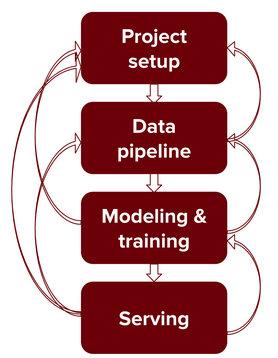
\includegraphics[scale=0.4]{GraphicFiles/theMLProjectFlow}
    \end{center}

    \tiny From \href{https://huyenchip.com/machine-learning-systems-design/design-a-machine-learning-system.html#design-a-machine-learning-system-dwGQI5R}{https://huyenchip.com/machine-learning-systems-design/design-a-machine-learning-system.html#design-a-machine-learning-system-dwGQI5R}

    \end{frame}}


    \section{Building the System}
    \label{sec:ourMLproject}

    \subsection{Project definition}
    \label{subsec:ourimplementation}

    \mode<beamer>{
    \begin{frame}
        \frametitle{Context}
        \label{context}
        %somecontext.tex



        \begin{block}{\textbf{Given the following}: \only<1,8>{\smallpencil{}}}
            \setbeamertemplate{itemize items}[ball]
            \begin{itemize}
                \uncover<2,8>{\item A global charitable donations platform \only<2>{\smallpencil{}}}
                \uncover<3,8>{\item Real-life anonymous transaction data \only<3>{\smallpencil{}}}
                \uncover<4,8>{\item No explicit user profiles \only<4>{\smallpencil{}}}
                \uncover<5,8>{\item Causes with categories and subcategories \only<5>{\smallpencil{}}}
                \uncover<6,8>{\item Collaborative filter (CF) \only<6>{\smallpencil{}}}
            \end{itemize}
        \end{block}

        \begin{block}{Build in the cloud}
            \begin{itemize}
                \uncover<7-8>{\item\alert{A prototype to make recommendations}\only<7>{\smallpencil{}}}
            \end{itemize}
        \end{block}
    \end{frame}}


    \subsection{Previous research}


    \mode<beamer>{
    \begin{frame}
        \frametitle{Donations related previous work}
        \label{previousresearch}
        % previousresearch.tex
        
        \vspace{3ex}
        
\includegraphics[scale=0.2]{GraphicFiles/DonationDashboard.png}
        
        \setbeamertemplate{itemize items}[ball]
        \begin{itemize}
            \item 59,000 ratings of 70 non-profit organizations from over 3,800 users, May 2009
            \item On-boarding interview to obtain user donation preferences
            \item Patented constant-time algorithm for recommendations: EigenTaste 2.0
        \end{itemize}
        \vspace{3ex}
    \end{frame}}


    \subsection{Inductive Bias}

    \mode<beamer>{
    \begin{frame}
        \frametitle{Algorithm selection}
        \label{recAlgoselection}
        % selectionRecAlgo.tex

    \setbeamertemplate{itemize items}[ball]

    Options for the basic recommendation algorithm:

    \begin{itemize}
        \item Content-based
        \item Item-based collaborative filter
        \item User-based collaborative filter
    \end{itemize}

    \vspace{2ex}

    Settled for Item-based CF due to:
    \begin{itemize}
        \item CF favours personalization and serendipity
        \item Lack of user profiles
    \end{itemize}
    \end{frame}}


    \mode<beamer>{
    \begin{frame}
        \frametitle{ML selection}
        \label{sparsity}
        %selectionMLsparsitycomplexity.tex

        \setbeamertemplate{itemize items}[ball]

        Strategies we considered:
        \begin{itemize}
            \item Dual-autoencoders
            \item Scalable SVD
        \end{itemize}

        \vspace{2ex}

        Settled for dual-autoencoders due to:
        \begin{itemize}
            \item Efficient use of memory
            \item Parallel pipeline design
        \end{itemize}
    \end{frame}}


    \mode<beamer>{
    \begin{frame}
        \frametitle{System metric selection}
        \label{relevance}
        % previousresearchrelevance.tex

    Could use:
    \begin{itemize}
        \item MAP
        \item Diversity
        \item Serendipity
        \item Novelty
        \item Coverage
    \end{itemize}

    \vspace{2ex}

    Chose MAP for simplicity

    \vspace{2ex}

    \tiny See
    K. Falk, Practical Recommender Systems. Shelter Island, NY: Manning Publications, 2019
    \vspace{1ex}
    Kaminskas, Marius and Bridge, and Derek, "Diversity, Serendipity, Novelty, and Coverage", ACM transactions on interactive intelligent systems, v.7, No. 1, pp. 1-14, 2016

    \end{frame}}

    \mode<beamer>{
    \begin{frame}
        \frametitle{Question}
        \label{question}
        %slideQuestions.tex

        
    \begin{block}{Given:}
		\setbeamertemplate{itemize items}[ball]
        \begin{itemize}
            \item Lack of explicit user profiles or ratings
            \item Sparsity: 
                \begin{itemize}
                    \item 24 million anonymous donations 
                    \item 165 thousand unique causes
                    \item Over 1.2 million users
                \end{itemize} 
        \end{itemize}
	\end{block}

    \vspace{1ex}
    \hspace{6em}    
    \begin{beamercolorbox}[sep=1em,wd=0.40\textwidth]{postit}
        How to make\\ \alert{relevant} recommendations?
   	\end{beamercolorbox}
    \vspace{3ex}

    \end{frame}}

    \section{Methodology}

    \subsection{Feature engineering}


    \mode<beamer>{
    \begin{frame}
        \frametitle{Generation of features}
        \label{featuregen}
        % featureeng.tex
    
        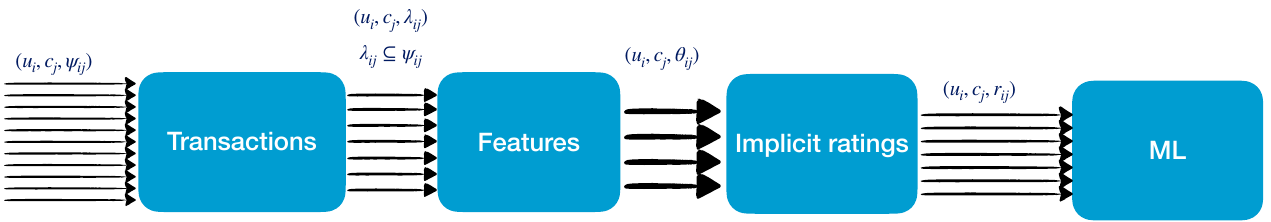
\includegraphics[scale=0.25]{GraphicFiles/FromTransactionsToFeatures.png}
    
    \begin{block}{To capture patterns from how users interact with causes}
        \begin{itemize}
            \item The set of transactions $\psi$ gets pre-processed into $\lambda$
            \item Then the set of features $\theta{}$ is computed
            \item Finally the set of implicit ratings, $r$, is generated
        \end{itemize}
    \end{block}
    \end{frame}}


    \mode<beamer>{
    \begin{frame}
        \frametitle{Features}
        \label{featuresdefinitions}
        % featuredefinitions.tex
    \begin{tabular}{cc}
        \begin{beamercolorbox}[sep=1em,wd=0.48\textwidth]{postit}
            FOCUS: how a user distributes their donation money among causes
   	    \end{beamercolorbox} &  \begin{beamercolorbox}[sep=1em,wd=0.49\textwidth]{postit}
   	        INTENSITY: capture the frequency of donations by a user to a category of causes
   	    \end{beamercolorbox}\\
        \begin{beamercolorbox}[sep=1em,wd=0.48\textwidth]{postit}
            IMPACT:  It is very similar to INTENSITY but in terms of money
        \end{beamercolorbox} &  \begin{beamercolorbox}[sep=1em,wd=0.49\textwidth]{postit}
            KIND: encodes the category of the cause donated to
        \end{beamercolorbox}
    \end{tabular}

    \end{frame}}


\subsection{Measuring relevance}


    \mode<beamer>{
    \begin{frame}
        \frametitle{Data set description}
        \label{dataset}
        % dataset.tex

% \begin{table}
\begin{center}
\tiny
    \begin{threeparttable}[b]
    \renewcommand{\arraystretch}{1.25}
    \caption{Statistics of data sets to make recommendations for donations to charities.}
    \label{tab:description_datasets}
    \centering
    \begin{tabular}{lrrrclrr} % an extra empty column introduced at column number 6 from left to right for aesthetics
        \toprule
        Dataset & \parbox[r][][t]{4em}{\raggedleft No. of users} & \parbox[r][][t]{4em}{\raggedleft No. of items} & \parbox[r][][t]{4.5em}{\raggedleft No. of ratings} & & \parbox[l][][t]{4em}{\raggedright Rating density} & \parbox[r][][t]{5em}{\raggedleft Avg. ratings per user} & \parbox[r]{5em}{\raggedleft Avg. ratings per item} \\
        \midrule
        % MovieLens-100K\tnote{1} & 943 & 1 682 & 100 000 & & 6.30\% & 106.04 & 59.45\\
        % MovieLens-1M\tnote{1} & 6 040 & 3 706 & 1 000 000 & & 4.47\% & 165.59 & 269.89\\
        Donations-Dashboard\tnote{1} & 3 133 & 70 & 57 517 & & 26.31\% & 18.42 & 851.9 \\
        Donations-1\tnote{2} & 9 397 & 2 711 & 24 417 & & 0.0958\% & 2.60 & 9.03 \\
        Donations-2\tnote{2} & 1 264 083 & 165 842 & 24 174 672 & &0.0115\% & 19.12 & 145.76 \\
        \bottomrule
    \end{tabular}
        \begin{tablenotes}
            % \item [1] The MovieLens Datasets: History and Context \cite{MovieLens2016}.
            \item [1] The Donation Dashboard data set: \href{http://dd.berkeley.edu/dataset/}{http://dd.berkeley.edu/dataset/}
            \item [2] Data used for this research.
        \end{tablenotes}
    \end{threeparttable}
\end{center}
% \end{table}

\small
\begin{block}{}
    Note the sparsity in rating density\footnote{The ratings per user per item} of the Donations-2 data set.
\end{block}
    \end{frame}}


    \mode<beamer>{
    \begin{frame}
        \frametitle{ML metrics}
        \label{mlmetrics}
        % measuringrelevance.tex


   
    \begin{block}{\textbf{Measuring what matters}: \only<1>{\smiley{}}}
        \alert<2>{For the machine learning components\ldots}\\
        \alert<3>{Regressor performance: RMSE, MAE} \action<3->{\cmark}\\
        \alert<4>{Classifier performance: precision, recall} \action<4->{\cmark}\\
        \alert<5>{Used during training and tuning via cross-validation} \action<5->{\cmark}\\
        \alert<6>{The goal is to generalize while avoiding over-fitting} \action<6->{\cmark}
    \end{block}
    \end{frame}}


    \mode<beamer>{
    \begin{frame}
        \frametitle{System performance metrics}
        \label{sysperformancemetrics}
        % measuringrecperf.tex

    \begin{block}{\textbf{System Performance}: }
        \alert<2>{A list of recommendations to a user\ldots}\\
        \alert<3>{is a ranked list of values} \\
        \alert<4>{and MAP is a more suitable metric.}\\
        \alert<5>{It requires that we can determine for each element}\\
        \alert<6>{of the list if it is relevant to the user} \only<6>{\alert{\faLightbulbO{}}} 
    \end{block}
    \end{frame}}


%    \mode<beamer>{
%    \begin{frame}
%        \frametitle{MAP}
%        \label{map}
%        % map.tex


    \begin{block}{\textbf{Mean Average Precision}: }
        \begin{itemize}
            \item Measures the average precision calculated up to each position in the ranked list and averaged over all the users.
            \item The precision at position $n$ in the list is determined by a binary variable, $r_n$
            \item $r_n=1$ if the category of the recommendation at position $n$ is among the ones chosen previously by the user, $r_n=0$ otherwise
        \end{itemize}
    \end{block}
%    \end{frame}}



\section{Results}


\subsection{Embedding size}


    \mode<beamer>{
    \begin{frame}
        \frametitle{Sensitivity to embedding size}
        \label{embeddingsizes}
        % embeddingsizes.tex

\begin{figure}
    \scriptsize
    \centering
    \begin{tikzpicture}
    \begin{axis}[mapfigs]
        \addplot[color=black,mark=diamond]
            coordinates {
            (3, 18.116666666666678)
            (5, 14.00277499999999)
            (7, 11.291706065759638)
            (9, 9.59428318185556)
            (11, 8.47514979493673)
            };\label{t3}
        \addplot[color=black, mark=triangle*]
            coordinates {
            (3, 16.953333333333323)
            (5, 13.151865186518658)
            (7, 10.679988586545726)
            (9, 9.030561344812489)
            (11, 7.953089315970777)
            };\label{t4}
        \node [draw,fill=white] at (rel axis cs: 0.732,0.762) {\shortstack[l]{
            \ref{t4} {\scriptsize scat/nc/256} \\
            \ref{t3} {\scriptsize scat/nc/512} }};
    \end{axis}
    \end{tikzpicture}
    \caption{\scriptsize Effect of the size of the cause embedding vectors on MAP at various values of top k for samples of 10,000 users. Key: scat=subcategories of causes used to compute features, nc=no feature for country of user, 256=embedding size, 512=embedding size.}
\end{figure}

    \end{frame}}

\subsection{Categories Vs. Subcategories}


    \mode<beamer>{
    \begin{frame}
        \frametitle{Cause categories Vs. subcategories}
        \label{catvssubcat}
        % catvssubcat.tex


\begin{figure}[htbp!]
    \scriptsize
    \centering
    \begin{tikzpicture}
    \begin{axis}[mapfigs]
        \addplot[color=black, mark=pentagon]
            coordinates {
            (3,25.78)(5,19.93)(7,16.02)(9,13.49)(11,11.97)
            };\label{plot:cat}
        \addplot[color=black, mark=triangle*]
            coordinates {
            (3, 16.953333333333323)
            (5, 13.151865186518658)
            (7, 10.679988586545726)
            (9, 9.030561344812489)
            (11, 7.953089315970777)
            };\label{plot:scat}
        \node [draw,fill=white] at (rel axis cs: 0.732,0.762) {\shortstack[l]{
            \ref{plot:cat} {\scriptsize cat/nc/256} \\
            \ref{plot:scat} {\scriptsize scat/nc/256} }};
    \end{axis}
    \end{tikzpicture}
    \caption{\scriptsize Effect of using categories or subcategories on MAP at different top k values for samples of 10,000 users. Key: cat=categories for feature computation, scat= subcategories instead of categories for feature computation, nc=no feature for country of user, 256=size of the cause embedding vectors.}
\end{figure}

    \end{frame}}

\subsection{User activity}


    \mode<beamer>{
    \begin{frame}
        \frametitle{Effect of user activity}
        \label{useractivity}
        % useractivity.tex

\begin{figure}
    \scriptsize
    \centering
    \begin{tikzpicture}
    \begin{axis}[mapfigs]
        \addplot[color=black, mark=square]
            coordinates {
            (3, 32.098888888888893)
            (5, 23.37503333333334)
            (7, 18.06751700680272)
            (9, 14.738761845437132)
            (11, 12.52077956822629)
            };\label{t1}
        \addplot[color=black, mark=*]
            coordinates {
            (3, 31.682507920626996)
            (5, 23.542875241715014)
            (7, 18.568244121075825)
            (9, 15.44195321111663)
            (11, 13.247696436388826)
            };\label{t5}
        \addplot[color=black, mark=x]
            coordinates {
            (3, 15.30333333333334)
            (5, 11.879900000000003)
            (7, 09.523418367346936)
            (9, 07.975152405917998)
            (11, 06.909317192197705)
            };\label{t7}
        \node [draw,fill=white] at (rel axis cs: 0.732,0.762) {\shortstack[l]{
            \ref{t7} {\scriptsize scat/1d/c/256} \\
            \ref{t1} {\scriptsize scat/55d/c/256} \\
            \ref{t5} {\scriptsize scat/100d/c/256} }};
    \end{axis}
    \end{tikzpicture}
    \caption{\scriptsize Effect of removing users with a minimum number of donations on MAP at various top k values for samples of 10,000 users. Key: scat= subcategories used for feature computation, c= country of the user as a feature, 1d=all users are included in the system, 55d=only users with 55 donations or more are included, 100d=only users with more than 100 donations are included.}
\end{figure}

    \end{frame}}


\subsection{Effect of setting the minimum donations per user}

    \mode<beamer>{
    \begin{frame}
        \frametitle{Transactions and users}
        \label{transacsusers}
        % paramtransacsusers.tex

\begin{figure}
    \scriptsize
    \centering
    \begin{tikzpicture}
    \pgfplotsset{set layers,
        log y ticks with fixed point/.style={
            yticklabel={
                \pgfkeys{/pgf/fpu=true}
                \pgfmathparse{exp(\tick)}%
                \pgfmathprintnumber[fixed relative, precision=3]{\pgfmathresult}
                \pgfkeys{/pgf/fpu=false}
            }
        }
    }
    \begin{axis}[donleft]
        \addplot[color=black, mark=square]
            coordinates {
            (1, 23.685965)
            (20, 20.114940)
            (40, 17.988919)
            (60, 15.876161)
            (80, 11.343628)
            (100, 10.067714)
            (150, 6.414618)
            (200, 4.764926)
            (300, 3.003430)
            (400, 1.988685)
            (500, 1.456254)
            };
            \label{pgfplots:nt}
    \end{axis}
    %
    \begin{semilogyaxis}[donlogright]
        \addplot[color=black, mark=*, domain=1:1500]
             coordinates {
             (1, 1215.453)
             (20, 252.239)
             (40, 179.381)
             (60, 135.338)
             (80, 66.413)
             (100, 51.967)
             (150, 22.565)
             (200, 13.240)
             (300, 5.981)
             (400, 3.007)
             (500, 1.814)
             };
        \label{pgfplots:users}
    \end{semilogyaxis}
    \end{tikzpicture}
    \caption{\scriptsize Number of transactions and number of users in the data set as a function of the minimum number of donations per user during the 2-year interval in the donations-2 data set.}
\end{figure}
    \end{frame}}



    \mode<beamer>{
    \begin{frame}
        \frametitle{Causes and companies}
        \label{paramcausescomps}
        % paramcausescomps.tex

\begin{figure}[htbp!]
    \scriptsize
    \centering
    \begin{tikzpicture}
    \pgfplotsset{set layers}
    \begin{axis}[comright]
        \addplot[color=black, mark=square]
            coordinates {
            (1, 413)
            (20, 353)
            (40, 307)
            (60,  273)
            (80,  243)
            (100, 215)
            (150, 187)
            (200, 168)
            (300, 118)
            (400, 93)
            (500, 73)
            };
            \label{pgfplots:cmp}
    \end{axis}
    %
    \begin{axis}[comleft]
        \addplot[color=black, mark=*]
             coordinates {
             (1, 165.318)
             (20, 97.436)
             (40, 77.945)
             (60, 66.287)
             (80, 53.647)
             (100, 47.181)
             (150, 35.339)
             (200, 27.750)
             (300, 19.043)
             (400, 13.630)
             (500, 10.445)
             };
        \label{pgfplots:cause}
    \end{axis}
    \end{tikzpicture}
    \caption{\scriptsize Number of causes and companies in the data set as a function of the minimum number of donations per user during the 2-year interval in the donations-2 data set.}
    \label{fig:number_of_companies_causes_vs_number_donations}
\end{figure}
    \end{frame}}

    \mode<beamer>{
    \begin{frame}
        \frametitle{Countries of users}
        \label{paramcountries}
        % paramcountries.tex

\begin{figure}
    \scriptsize
    \centering
    \begin{tikzpicture}
    \pgfplotsset{set layers}
    \begin{axis}[cntyleft]
        \addplot[color=black, mark=*]
             coordinates {
                 (1, 47)
                 (20, 41)
                 (40, 35)
                 (60,  29)
                 (80,  21)
                 (100, 15)
                 (150, 9)
                 (200, 8)
                 (300, 6)
                 (400, 6)
                 (500, 4)
            };
        \label{pgfplots:usrcnty}
    \end{axis}
    \end{tikzpicture}
    \caption{\scriptsize Number of user countries in the data set as a function of the minimum number of donations per user during the 2-year interval in the donations-2 data set.}
\end{figure}
    \end{frame}}


\section{Conclusions}


\mode<beamer>{
    \begin{frame}
        \frametitle{Conclusions}
        \label{conclusionsclassification}
    % conclusions.tex

\setbeamertemplate{itemize items}[ball]
\begin{itemize}
    \item Successfully used inferred user profiles via implicit ratings
	\item Using finer cause classifications increases relevance
    \item Controlling for minimum number of donations improves MAP
    \item An empirical threshold for user donations seems reasonable to max MAP at any $k$
\end{itemize}
\vspace{3ex}
    \end{frame}
}

\section{Acknowledgements}

\mode<beamer>{
    \begin{frame}
        \frametitle{Acknowledgements}
        \label{acknowledgments}
    % ackwoledgements.tex

Special thanks for funding and supporting this research:

\begin{itemize}
    \item The University of Calgary, Software Engineering Program
	\item \href{https://www.mitacs.ca/en/programs/accelerate}{MITACS Accelerate}
    \item \href{https://benevity.com/}{Benevity, Inc.}
\end{itemize}


    \end{frame}
}

    Thanks to Benevity and MITACS for funding this research and to the University of Calgary the Master of Engineering program in Software Engineering that gave us the principles to tackle this subject.

    %----------------------------------------------------------------------------------------
    \begin{figure}[!htbp]
        \begin{center}
            \framebox{\includeslide[width=0.45\textwidth]{acknowledgments}}
            \caption{Acknowledgments}
            \label{fig:ackwoledgements}
        \end{center}
    \end{figure}
    %----------------------------------------------------------------------------------------

%\section*{Additional Support slides}
%    \mode<all>{
%        \usebackgroundtemplate{%
%        
\includegraphics[width=\paperwidth,height=\paperheight]{GraphicFiles/WhiteBackGround.jpg}%
%        }% this background gets applied for now on in every frame unless otherwise specified,
%        % e.g. by using the option [plain] in the frame environment
%    }
%
%
%    \mode<beamer>{
%    \begin{frame}[noframenumbering]
%        \frametitle{Data flow\\System level}
%        \label{dataflowsystem}
%        % systemdataflow.tex
    \vspace{-9ex}
    \begin{columns}[onlytextwidth,T]
        \column{7em}
        \column{\linewidth-7em}
        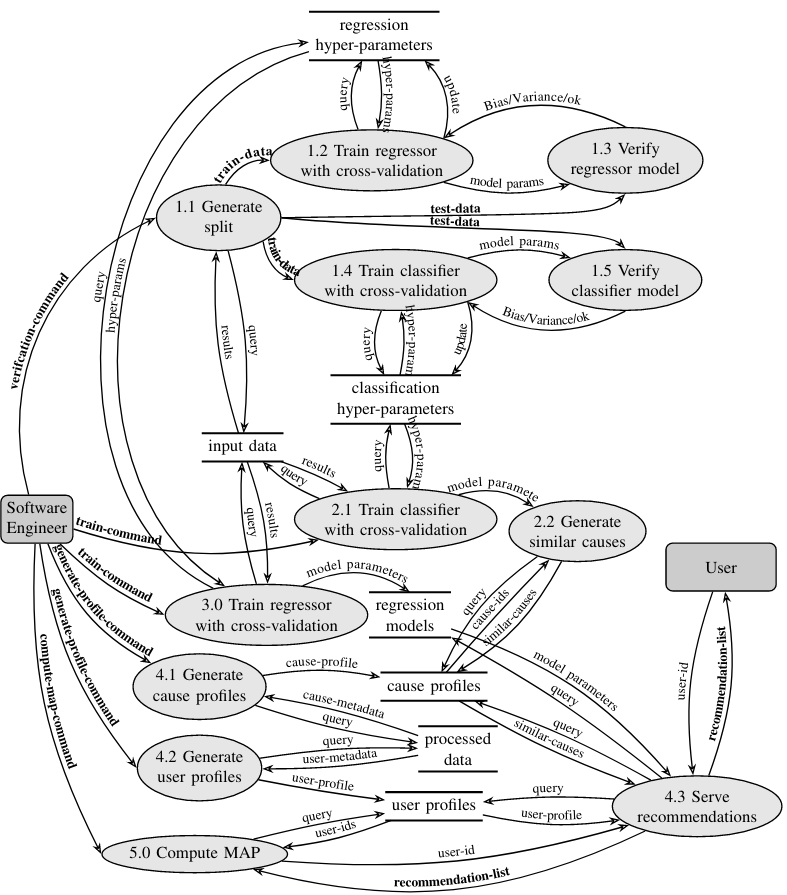
\includegraphics[scale=0.28]{GraphicFiles/DataFlowSystemLevelAfterPreProcessing.png}
    \end{columns}
         
%    \end{frame}
%    }
%
%    A data flow graph for the recommendation system that did not make it to the paper for lack of space.
%    It shows the Software Engineer and the user as the two main agents external to the system.
%    Paths 1 through 3 are used to prepare the system via machine learning.
%    Path 4 addresses calculating a recommendation list.
%    Path 5 has to do with computing MAP for system performance assessment.



%    %----------------------------------------------------------------------------------------
%    \begin{figure}[!htbp]
%        \begin{center}
%            \framebox{\includeslide[width=0.45\textwidth]{dataflowsystem}}
%            \caption{Data flow at system level}
%            \label{fig:dataflowsystem}
%        \end{center}
%    \end{figure}
%    %----------------------------------------------------------------------------------------

%    \mode<all>{
%        \usebackgroundtemplate{%
%          
\includegraphics[width=\paperwidth,height=\paperheight]{GraphicFiles/MeetUpData4GoodBackground.png}%
%        }% this background gets applied for now on in every frame unless otherwise specified,
%        % e.g. by using the option [plain] in the frame environment
%    }

\end{document}
